\documentclass{article}
\usepackage[utf8]{inputenc}
\usepackage{amsmath}
\title{Report Lab DC: Digital Systems}
\author{Henning Schei}
\date{March 2016}
\usepackage{natbib}
\usepackage{graphicx}
\usepackage{listings}
\usepackage{color}
\usepackage{float}
\definecolor{dkgreen}{rgb}{0,0.6,0}
\definecolor{gray}{rgb}{0.5,0.5,0.5}
\definecolor{mauve}{rgb}{0.58,0,0.82}

\lstset{frame=tb,
  language=VHDL,
  aboveskip=3mm,
  belowskip=3mm,
  showstringspaces=false,
  columns=flexible,
  basicstyle={\small\ttfamily},
  numbers=none,
  numberstyle=\tiny\color{gray},
  keywordstyle=\color{blue},
  commentstyle=\color{dkgreen},
  stringstyle=\color{mauve},
  breaklines=true,
  breakatwhitespace=true,
  tabsize=3
}
\begin{document}

\maketitle


\section{Refinement of a VHDL model for synthesis}

\begin {itemize}
\item The target clock period is 2.0 nm, so the clock freq is 1/2.0 = 5e+8 = 500 MHz.
\item The input and output delay is 0.5 ns
\item The synthesis gives the following errors
Error:  ../g1.vhd:27: WAIT statement inside FOR loop is not supported. (ELAB-996)
Error:  ../g1.vhd:27: WAIT statement inside FOR loop is not supported. (ELAB-996)

There are wait statements on several occations in the process. These lines needs to be rewritten to be synthesizable. I did the following.


\begin{lstlisting}
p: process(clk)
  begin
    -- First, if the condition to start a macro-cycle does not hold, synchronize
    -- on a rising edge of clock where a is active. Else, start a macro-cycle.

    if clk = '1' and clk'event then
      if a = '1' then
        -- if not (clk = '1' and clk'event and a = '1') then
        --  wait until clk = '1' and clk'event and a = '1';
        -- end if;
        s_local <= '1'; -- a macro-cycle starts (set s_local)
        for i in 4 downto 0 loop -- a macro-cycle is made of 5 sequences
          for j in 1 to 2 ** i loop -- wait for 2^i cycles

          end loop;
          s_local <= not s_local; -- invert s_local
        end loop;
      end if;
    end if;
  end process p;
\end{lstlisting}

\item 
\begin{figure}[H]
\begin {center}
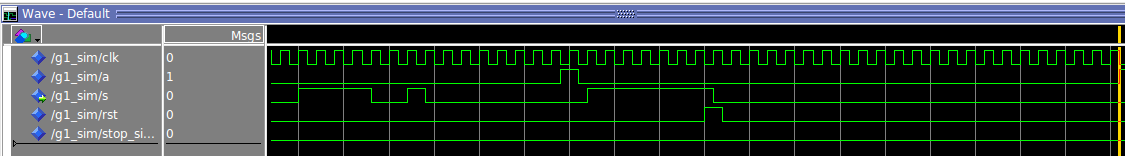
\includegraphics[scale=0.4]{syncrst.png}
\caption{wave diagram showing sync reset}
\end{center}
\end{figure}








\end {itemize}



\section {Synthesis reports}
\begin{itemize}
\item The silicon area of the synthesized circuit is 102 $\mu m^2$.
\item According to the model, it should be 5 DFFs. And it's the same as in the html page. 
\item   
\end{itemize}


\end{document}

